\documentclass[10pt,a4paper,twoside]{article}%ustalasz jaki typ dokumentu i właściwości

\usepackage[polish]{babel} % ustawianie języka polskiego
\usepackage[colorlinks=false,linkcolor=green,urlcolor=green,citecolor=green]{hyperref}%hiperłącza ogólnego rodzaju
\hypersetup{pdftitle=Sprawozdanie PSIO}

\usepackage{pdfpages} % importowanie plików z pdfa
\usepackage{amsmath} % do wstawiania macierz itp
\usepackage{graphicx} % wstawianie zdjęć
% \usepackage[utf8]{inputenc} % niepotrzebne bo lualatex
\usepackage[T1]{fontenc} % niepotrzebne bo lualatex
\usepackage[left=2cm,right=2cm,top=2cm,bottom=2cm, footskip=1cm,
columnsep=1.5cm % odstęp między kolumnami
]{geometry}%marginesy

\usepackage{listings} % punktowanie
% \usepackage{indentfirst} % dawanie akapitu na początku
\usepackage{caption} % podpisy
\usepackage{subcaption} % podpisy do subfigure
\usepackage{siunitx} % jednostki si
\usepackage{minted} % ładne kody naprzyklad matlaba
\setminted{linenos=true,frame=none,breaklines=true,breaksymbolleft=,style=vs,bgcolor={gray!10}}

\usepackage{textcase}

\usepackage[polish,nameinlink]{cleveref} % dobre prefiksy przed etykietą i język
\usepackage{cprotect}

\usepackage{fontspec}
% \setmainfont[Ligatures=TeX]{Georgia}
% \setsansfont[Ligatures=TeX]{Arial}
\usepackage{parskip} % usunięcie tab na początku akapitu
\usepackage{newfloat} % aby można było ładnie wstawić elementy typu zdjecie, kod itp

%%% rysowanie wykresów %%% ale w ciul to trudne więc app.diagrams.net
\usepackage{tikz}
\usetikzlibrary{shapes.geometric, arrows, positioning}

% % % SVG import
\usepackage{svg}
\usepackage{import}
\usepackage{xifthen}
\usepackage{transparent}

% \usepackage{mdframed} % ramki
\usepackage[framemethod=TikZ]{mdframed}
\mdfsetup{%
middlelinecolor=red,
middlelinewidth=1pt,
   backgroundcolor=gray!20,
   roundcorner=10pt}

\usepackage{enumitem} % podpunkty customowe

\usepackage{pgfplots}[compat=1.18] % wykresy

\boldmath%pogrubiona matma

%%%%%%%%%%%%%% koniec pakietów %%%%%%%%%%%%%%%%%%%%%%%%%%%

\title{Fajny ten tytuł}%tytuł
\date{\today}%%data
\author{Janusz Chmaruk}%autor
\setcounter{secnumdepth}{3}%głębokość liczenia roździałów

% PRZYKŁAD LICZNIKA ZADAŃ
\newcounter{zadanie}
\newenvironment{zadanie}[1][]{
   \refstepcounter{zadanie}
   \subsection*{Zadanie \thezadanie#1}
   \addcontentsline{toc}{subsection}{Zadanie \thezadanie#1} % dodanie do spisu treści
}{}

% PRZYKŁAD LICZNIKA ROZWIĄZAŃ
\newcounter{rozwiazanie}
\newenvironment{rozwiazanie}[1][]{
   \refstepcounter{rozwiazanie}
   \subsection*{Rozwiazanie zadania \therozwiazanie#1}
   \addcontentsline{toc}{subsection}{Rozwiazanie zadania \therozwiazanie#1} % dodanie do spisu treści
}{}


% DŁUGIE LISTINGI
\newenvironment{longlisting}{\captionsetup{type=listing}}{}

\newcounter{licznikFigure}
\newcommand{\CC}{\refstepcounter{licznikFigure}\caption*{figure \thelicznikFigure}}


%%%%%%%%%%%%%%%%%%%%%%%%%%%%%%%%%%%%%%%%%%%%%%%%%%%%%%%%%%%%%%%
%%%%%%%%%%%%%%%%%%%%%%%%%%%%%%%%%%%%%%%%%%%%%%%%%%%%%%%%%%%%%%%
%%%%%%% TU SIE ZACZYNA PISANIE PLIKU %%%%%%%%%%%%%%%%%%%%%%%%%%
%%%%%%%%%%%%%%%%%%%%%%%%%%%%%%%%%%%%%%%%%%%%%%%%%%%%%%%%%%%%%%%
%%%%%%%%%%%%%%%%%%%%%%%%%%%%%%%%%%%%%%%%%%%%%%%%%%%%%%%%%%%%%%%

\begin{document}

% \null
\includepdf[pages={1}]{Szablon_Projektu.pdf}
\newpage

\tableofcontents
% \newpage

\section{Cel ćwiczenia}
Celem ćwiczenia jest poznanie znaczenia binaryzacji w praktyce przetwarzania i analizy obrazów. Nabycie praktycznych umiejętności: stosowania odpowiednik technik i metod binaryzacji oraz opisu własności histogramów obrazu cyfrowego. Zapoznanie się z podstawowymi przekształceniami kontekstowymi obrazów głównie z przekształceniami morfologicznymi.

\section{Zadania do realizacji}

\begin{zadanie}
    Wczytać dowolny obraz (RGB) a następnie przekształcić go do postaci obrazu binarnego:

    \begin{enumerate} \item BW = im2bw(I, level), BW = im2bw(X, map, level), BW = im2bw(RGB, level) level- poziom/próg binaryzacji określić na podstawie histogramu obrazu w odcieniach szarości -nasycenie/odcień szarości o największej liczbie pikseli (ponadto opisać jakie informacje są zawarte na histogramie) \item BW=imbinarize(I), BW=imbinarize(I,method), BW=imbinarize(I,T), BW= imbinarize(I,`adaptive',Name,Value) \item dla obrazu w odcieniach szarości wykorzystać funkcję graythresh \item dla obrazu w odcieniach szarości dokonać binaryzacji: \item na podstawie wartości z zakresu +/-30\% nasycenia/odcieni szarości o największej liczbie pikseli --- wartość progu oszacowana na podstawie histogramu (binaryzacja z podwójnym ograniczeniem) \item * podziel obraz na 16 bloków, dla każdego bloku wyznacz wartość progu binaryzacji i przeprowadź binaryzację, następnie scal obraz. Uzasadnij dobór progu binaryzacji. Opisz wyniki. \end{enumerate}

    Dla wybranego obrazu dokonać wyrównywania histogramu (funkcja histeq). Przedstawić i opisać różnice w odniesieniu do oryginalnego obrazu i jego histogramu oraz obrazu oryginalnego (całego) po operacji wyrównywania histogramu.
\end{zadanie}


\begin{zadanie}
    Operacje morfologiczne. Stwórz obraz w dowolnym programie graficznym, na którym są takie elementy jak: zatoczki w obiektach, inicjały (po trzy pierwsze litery imienia i nazwiska wybranej osoby z grupy), wypustki dla dowolnego obiektu, dwa stykające obiekty, kilka obiektów o różnym kolorze, kształcie i wielkości.

\begin{enumerate}
    \item za pomocą funkcji `strel' wygenerować 4 wybranych elementów strukturalnych. Opisać je skrótowo, przedstawić obrazy i postać macierzową. sel=strel(`pair', [2,-1]); figure; imshow(getnhood(sel),`InitialMagnification', `fit'); 
    \item dla uzyskanego obrazu dokonać operacji: erozji, dylatacji, zamknięcia, otwarcia z uwzględnieniem doboru elementu strukturalnego (pokazać na rysunku, opisać, uzasadnić); 
    \item dla wybranego fragmentu obrazu - inicjały (do wycięcia można użyć funkcji imcrop) dokonać operacji binaryzacji, a następnie wyznaczyć gradient morfologiczny tj.: - różnicę między obrazem wejściowym, a wynikiem jego erozji; - różnicę między wynikiem dylatacji, a obrazem wejściowym; - połowę różnicy między wynikiem dylatacji, a erozji.
\end{enumerate}

\end{zadanie}

\section{Zrealizowane zadania}

\begin{rozwiazanie}
    
    \begin{longlisting}
        \begin{minted}{matlab}
% Usunięcie wszystkich zmiennych z przestrzeni roboczej, zamknięcie wszystkich otwartych okien
clc; close all;

% Wczytanie obrazu
Im = imread('Im.jpg');

% Konwersja obrazu do skali szarości
Im_gray = rgb2gray(Im);

% Konwersja obrazu RGB do obrazu indeksowanego
[Im_ind, cmap] = rgb2ind(Im, 2048);

% a
% Wykreślenie histogramu obrazu w skali szarości
histogram(Im_gray);

% Binaryzacja obrazu
BW1 = im2bw(Im, 0.65); BW2 = im2bw(Im_ind, cmap, 0.65);
BW3 = im2bw(Im_gray, 0.65);

% Wyświetlenie wyników binaryzacji
figure(1); imshow(BW1); title('(Im, 0.65)');disp('exportgraphics'); exportgraphics(gcf,'myVectorFile1.pdf','BackgroundColor','none','ContentType','vector')
figure(2); imshow(BW2); title('(Im ind, cmap, 0.65)');disp('exportgraphics'); exportgraphics(gcf,'myVectorFile2.pdf','BackgroundColor','none','ContentType','vector')
figure(3); imshow(BW3); title('(Im gray, 0.65)');disp('exportgraphics'); exportgraphics(gcf,'myVectorFile3.pdf','BackgroundColor','none','ContentType','vector')

% b
% Binaryzacja obrazu za pomocą różnych metod
BIN1 = imbinarize(Im);
BIN2 = imbinarize(Im, 'global'); BIN2_a = imbinarize(Im, 'adaptive');
BIN3 = imbinarize(Im, 0.6);
BIN4 = imbinarize(Im, 'adaptive', 'Sensitivity', 0.5, ...
    'ForegroundPolarity', 'dark');
BIN4_b = imbinarize(Im, 'adaptive', 'Sensitivity', 0.5, ...
    'ForegroundPolarity', 'bright');
BIN4_3 = imbinarize(Im, 'adaptive', 'Sensitivity', 0.3, ...
    'ForegroundPolarity', 'dark');
BIN4_7 = imbinarize(Im, 'adaptive', 'Sensitivity', 0.7, ...
    'ForegroundPolarity', 'dark');

% Wyświetlenie wyników binaryzacji
figure(4); imshow(BIN1(:,:,1)); title(' domyslne dzialanie imbinarize');disp('exportgraphics'); exportgraphics(gcf,'myVectorFile4.pdf','BackgroundColor','none','ContentType','vector')
figure(5); imshow(BIN2(:,:,1)); title(' metoda globalna ');disp('exportgraphics'); exportgraphics(gcf,'myVectorFile5.pdf','BackgroundColor','none','ContentType','vector')
figure(6); imshow(BIN2_a(:,:,1)); title(' metoda adaptacyjna ');disp('exportgraphics'); exportgraphics(gcf,'myVectorFile6.pdf','BackgroundColor','none','ContentType','vector')
figure(7); imshow(BIN3(:,:,1)); title(' granica 0.6');disp('exportgraphics'); exportgraphics(gcf,'myVectorFile7.pdf','BackgroundColor','none','ContentType','vector')
figure(8); imshow(BIN4(:,:,1)); title([' metoda adaptacyjna, wspolczynnik ' ...
    'czulosci 0.5, piksele tla ciemne  ']);disp('exportgraphics'); exportgraphics(gcf,'myVectorFile8.pdf','BackgroundColor','none','ContentType','vector')
figure(9); imshow(BIN4_b(:,:,1)); title([' metoda adaptacyjna, wspolczynnik ' ...
    'czulosci 0.5, piksele tla jasne  ']);disp('exportgraphics'); exportgraphics(gcf,'myVectorFile9.pdf','BackgroundColor','none','ContentType','vector')
figure(10); imshow(BIN4_3(:,:,1)); title([' metoda adaptacyjna, wspolczynnik ' ...
    'czulosci 0.3, piksele tla ciemne  ']);disp('exportgraphics'); exportgraphics(gcf,'myVectorFile10.pdf','BackgroundColor','none','ContentType','vector')
figure(11); imshow(BIN4_7(:,:,1)); title([' metoda adaptacyjna, wspolczynnik ' ...
    'czulosci 0.7, piksele tla ciemne  ']);disp('exportgraphics'); exportgraphics(gcf,'myVectorFile11.pdf','BackgroundColor','none','ContentType','vector')

% c
% Wyznaczenie progu binaryzacji za pomocą metody Otsu
level = graythresh(Im_gray); % 0.635

% Binaryzacja obrazu z wykorzystaniem wyznaczonego progu
BW_gray = imbinarize(Im_gray,level);

% Wyświetlenie wyniku
figure(12); imshow(BW_gray); title('z graythresh');disp('exportgraphics'); exportgraphics(gcf,'myVectorFile12.pdf','BackgroundColor','none','ContentType','vector')

% d1
% Modyfikacja obrazu w skali szarości za pomocą progowania na poziomie pikseli
sizeim = size(Im_gray);
Im_gray_bin = Im_gray;
for i = 1:sizeim(1)
    for j = 1:sizeim(2)
        if(Im_gray_bin(i,j) > 100 && Im_gray_bin(i,j) < 200)
            for k=0:5
                kk = 5-k;
                if Im_gray_bin(i,j) > 100 + kk*20
                    Im_gray_bin(i,j) = 100 + kk*20;
                    break
                end
            end
        end
    end
end

% Wyświetlenie wyniku oraz histogramu
figure(13); imshow(Im_gray_bin);disp('exportgraphics'); exportgraphics(gcf,'myVectorFile13.pdf','BackgroundColor','none','ContentType','vector')
figure(14); histogram(Im_gray_bin); grid on;disp('exportgraphics'); exportgraphics(gcf,'myVectorFile14.pdf','BackgroundColor','none','ContentType','vector')

% d2
% Wyznaczenie histogramu oraz najczęściej występującej wartości natężenia
[pixelCounts, grayLevels] = imhist(Im_gray);
[~, idx] = max(pixelCounts(:));

% Progowanie obrazu na podstawie najczęściej występującej wartości natężenia
l_lim = idx - (idx * 0.3); r_lim = idx + (idx * 0.3);
Im_gray_bin2 = Im_gray;
for i = 1:sizeim(1)
    for j = 1:sizeim(2)
        if(Im_gray_bin2(i,j) > l_lim && Im_gray_bin2(i,j) < r_lim)
            Im_gray_bin2(i,j) = 1;
        else
            Im_gray_bin2(i,j) = 0;
        end
    end
end

% Wyświetlenie wyniku oraz histogramu
figure(15); imshow(Im_gray_bin2, [0 1]);disp('exportgraphics'); exportgraphics(gcf,'myVectorFile15.pdf','BackgroundColor','none','ContentType','vector')
figure(16); histogram(Im_gray_bin2); grid on;disp('exportgraphics'); exportgraphics(gcf,'myVectorFile16.pdf','BackgroundColor','none','ContentType','vector')

% 2
% Wyrównanie histogramu
Im_wyr =  histeq(Im_gray);

% Wyświetlenie obrazu oryginalnego, po wyrównaniu histogramu oraz histogramu obrazu po wyrównaniu
figure(17); imshow(Im_gray); title('Orginal');disp('exportgraphics'); exportgraphics(gcf,'myVectorFile17.pdf','BackgroundColor','none','ContentType','vector')
figure(18); imshow(Im_wyr); title('Po histeq');disp('exportgraphics'); exportgraphics(gcf,'myVectorFile18.pdf','BackgroundColor','none','ContentType','vector')
figure(19); histogram(Im_wyr); grid on;disp('exportgraphics'); exportgraphics(gcf,'myVectorFile19.pdf','BackgroundColor','none','ContentType','vector')
        \end{minted}
        
    \end{longlisting}Ten kod MATLAB-a jest używany do przetwarzania obrazu. Po wczytaniu obrazu, wykonuje szereg operacji, w tym konwersję do skali szarości, binaryzację obrazu za pomocą różnych technik, wyznaczanie progu binaryzacji za pomocą metody Otsu, modyfikację obrazu w skali szarości przez progowanie na poziomie pikseli, wyrównanie histogramu i prezentację wyników na histogramach i jako obrazy.
\end{rozwiazanie}
\begin{rozwiazanie}
    

\begin{longlisting}
    \begin{minted}{matlab}
% Usuwanie wszystkich zmiennych z przestrzeni roboczej, czyszczenie konsoli i zamknięcie wszystkich otwartych okien
clc; clear all; close all;

% Wczytanie obrazu
obr1 = imread("Im.jpg");

%% Operacje morfologiczne
close all;
obr3 = imread('Bez tytułu.png');

% Tworzenie struktur elementarnych
prostokat = strel('rectangle',[16,16]);
diament = strel('diamond',8);
dysk = strel('disk',8);
oktagon = strel('octagon',9);

% Wyświetlanie struktur elementarnych
figure(20);
subplot(2, 2, 1), imshow(getnhood(prostokat), 'InitialMagnification', 'fit') , title('prostokat');
subplot(2, 2, 2), imshow(getnhood(diament), 'InitialMagnification', 'fit') ;title('diament');
subplot(2, 2, 3), imshow(getnhood(dysk), 'InitialMagnification', 'fit') ;title('dysk');
subplot(2, 2, 4), imshow(getnhood(oktagon), 'InitialMagnification', 'fit') ;title('oktagon');
disp('exportgraphics'); exportgraphics(gcf,'myVectorFile20.pdf','BackgroundColor','none','ContentType','vector');
%% Tworzenie operacji erozji, dylatacji, zamknięcia i otwarcia
close all; clc;
obr2 = imread('Bez tytułu.png'); % Wczytanie obrazu "obr2"

% Tworzenie struktury elementarnej typu "disk" o rozmiarze 3
se = strel('disk', 3);

% Erozja
ero_obr2 = imerode(obr2, se);

% Dylatacja
dyl_obr2 = imdilate(obr2, se);

% Zamknięcie
zamk_obr2 = imclose(obr2, se);

% Otwarcie
otw_obr2 = imopen(obr2, se);

% Wyświetlanie obrazów i ich operacji
figure(21),imshow(obr2), title('Obraz "obr2"');disp('exportgraphics'); exportgraphics(gcf,'myVectorFile21.pdf','BackgroundColor','none','ContentType','vector');
figure(22),imshow(ero_obr2), title('Erozja');disp('exportgraphics'); exportgraphics(gcf,'myVectorFile22.pdf','BackgroundColor','none','ContentType','vector');
figure(23),imshow(dyl_obr2), title('Dylatacja');disp('exportgraphics'); exportgraphics(gcf,'myVectorFile23.pdf','BackgroundColor','none','ContentType','vector');
figure(24),imshow(zamk_obr2), title('Zamknięcie');disp('exportgraphics'); exportgraphics(gcf,'myVectorFile24.pdf','BackgroundColor','none','ContentType','vector');
figure(25),imshow(otw_obr2), title('Otwarcie');disp('exportgraphics'); exportgraphics(gcf,'myVectorFile25.pdf','BackgroundColor','none','ContentType','vector');

%% Wyznaczanie gradientu morfologicznego
inicjaly = imcrop(obr3, [778,38, 200 , 100]);
%778,38 - 928,146
figure(26); imshow(inicjaly); title('Obraz oryginalny')

% Erozja
inicjaly_e = imerode(inicjaly, dysk);

% Dylatacja
inicjaly_d = imdilate(inicjaly, dysk);
disp('exportgraphics'); exportgraphics(gcf,'myVectorFile26.pdf','BackgroundColor','none','ContentType','vector');
% Wyświetlanie obrazów po erozji i dylatacji
figure(27); imshow(inicjaly_d), title('dylatacja');disp('exportgraphics'); exportgraphics(gcf,'myVectorFile27.pdf','BackgroundColor','none','ContentType','vector');
figure(28); imshow(inicjaly_e), title('erozja');disp('exportgraphics'); exportgraphics(gcf,'myVectorFile28.pdf','BackgroundColor','none','ContentType','vector');

% Obliczanie gradientu morfologicznego różnymi metodami
A = inicjaly - inicjaly_e;
B = inicjaly_d - inicjaly;
C = 0.5 * (inicjaly_d - inicjaly_e);

% Wyświetlanie gradientów morfologicznych
figure(29); imshow(A); title(' wej - erozja ');disp('exportgraphics'); exportgraphics(gcf,'myVectorFile29.pdf','BackgroundColor','none','ContentType','vector');
figure(30); imshow(B); title(' dylatacja - wej ');disp('exportgraphics'); exportgraphics(gcf,'myVectorFile30.pdf','BackgroundColor','none','ContentType','vector');
figure(31); imshow(C); title(' dylatacja - erozja ');disp('exportgraphics'); exportgraphics(gcf,'myVectorFile31.pdf','BackgroundColor','none','ContentType','vector');

    \end{minted}
\end{longlisting}Kod ten demonstruje podstawowe operacje morfologiczne na obrazach, takie jak erozja, dylatacja, otwarcie i zamknięcie, a także oblicza gradient morfologiczny obrazu. Operacje te są często używane w przetwarzaniu obrazów do różnych celów, takich jak usuwanie szumów, separacja obiektów, ekstrakcja krawędzi itp.
\end{rozwiazanie}

\begin{figure}[H]
    \centering
    \includegraphics[width=0.8\linewidth]{kod matlab/myVectorFile1.pdf}
    \caption{figure(1)}
    \label{fig:obr1}
\end{figure}

\begin{figure}[H]
    \centering
    \includegraphics[width=0.8\linewidth]{kod matlab/myVectorFile2.pdf}
\caption{figure(2)}
    \label{fig:obr1}
\end{figure}

\begin{figure}[H]
    \centering
    \includegraphics[width=1\linewidth]{kod matlab/myVectorFile3.pdf}
\caption{figure(3)}
\end{figure}

\begin{figure}[H]
    \centering
    \includegraphics[width=1\linewidth]{kod matlab/myVectorFile4.pdf}
\caption{figure(4)}
    \label{fig:obr1}
\end{figure}

\begin{figure}[H]
    \centering
    \includegraphics[width=1\linewidth]{kod matlab/myVectorFile5.pdf}
\caption{figure(5)}
    \label{fig:obr1}
\end{figure}

\begin{figure}[H]
    \centering
    \includegraphics[width=1\linewidth]{kod matlab/myVectorFile6.pdf}
\caption{figure(6)}
    \label{fig:obr1}
\end{figure}

\begin{figure}[H]
    \centering
    \includegraphics[width=1\linewidth]{kod matlab/myVectorFile7.pdf}
\caption{figure(7)}
    \label{fig:obr1}
\end{figure}

\begin{figure}[H]
    \centering
    \includegraphics[width=1\linewidth]{kod matlab/myVectorFile8.pdf}
\caption{figure(8)}
    \label{fig:obr1}
\end{figure}

\begin{figure}[H]
    \centering
    \includegraphics[width=1\linewidth]{kod matlab/myVectorFile9.pdf}
\caption{figure(9)}
    \label{fig:obr1}
\end{figure}

\begin{figure}[H]
    \centering
    \includegraphics[width=1\linewidth]{kod matlab/myVectorFile10.pdf}
\caption{figure(10)}
    \label{fig:obr1}
\end{figure}

\begin{figure}[H]
    \centering
    \includegraphics[width=1\linewidth]{kod matlab/myVectorFile11.pdf}
\caption{figure(11)}
    \label{fig:obr1}
\end{figure}

\begin{figure}[H]
    \centering
    \includegraphics[width=1\linewidth]{kod matlab/myVectorFile12.pdf}
\caption{figure(12)}
    \label{fig:obr1}
\end{figure}

\begin{figure}[H]
    \centering
    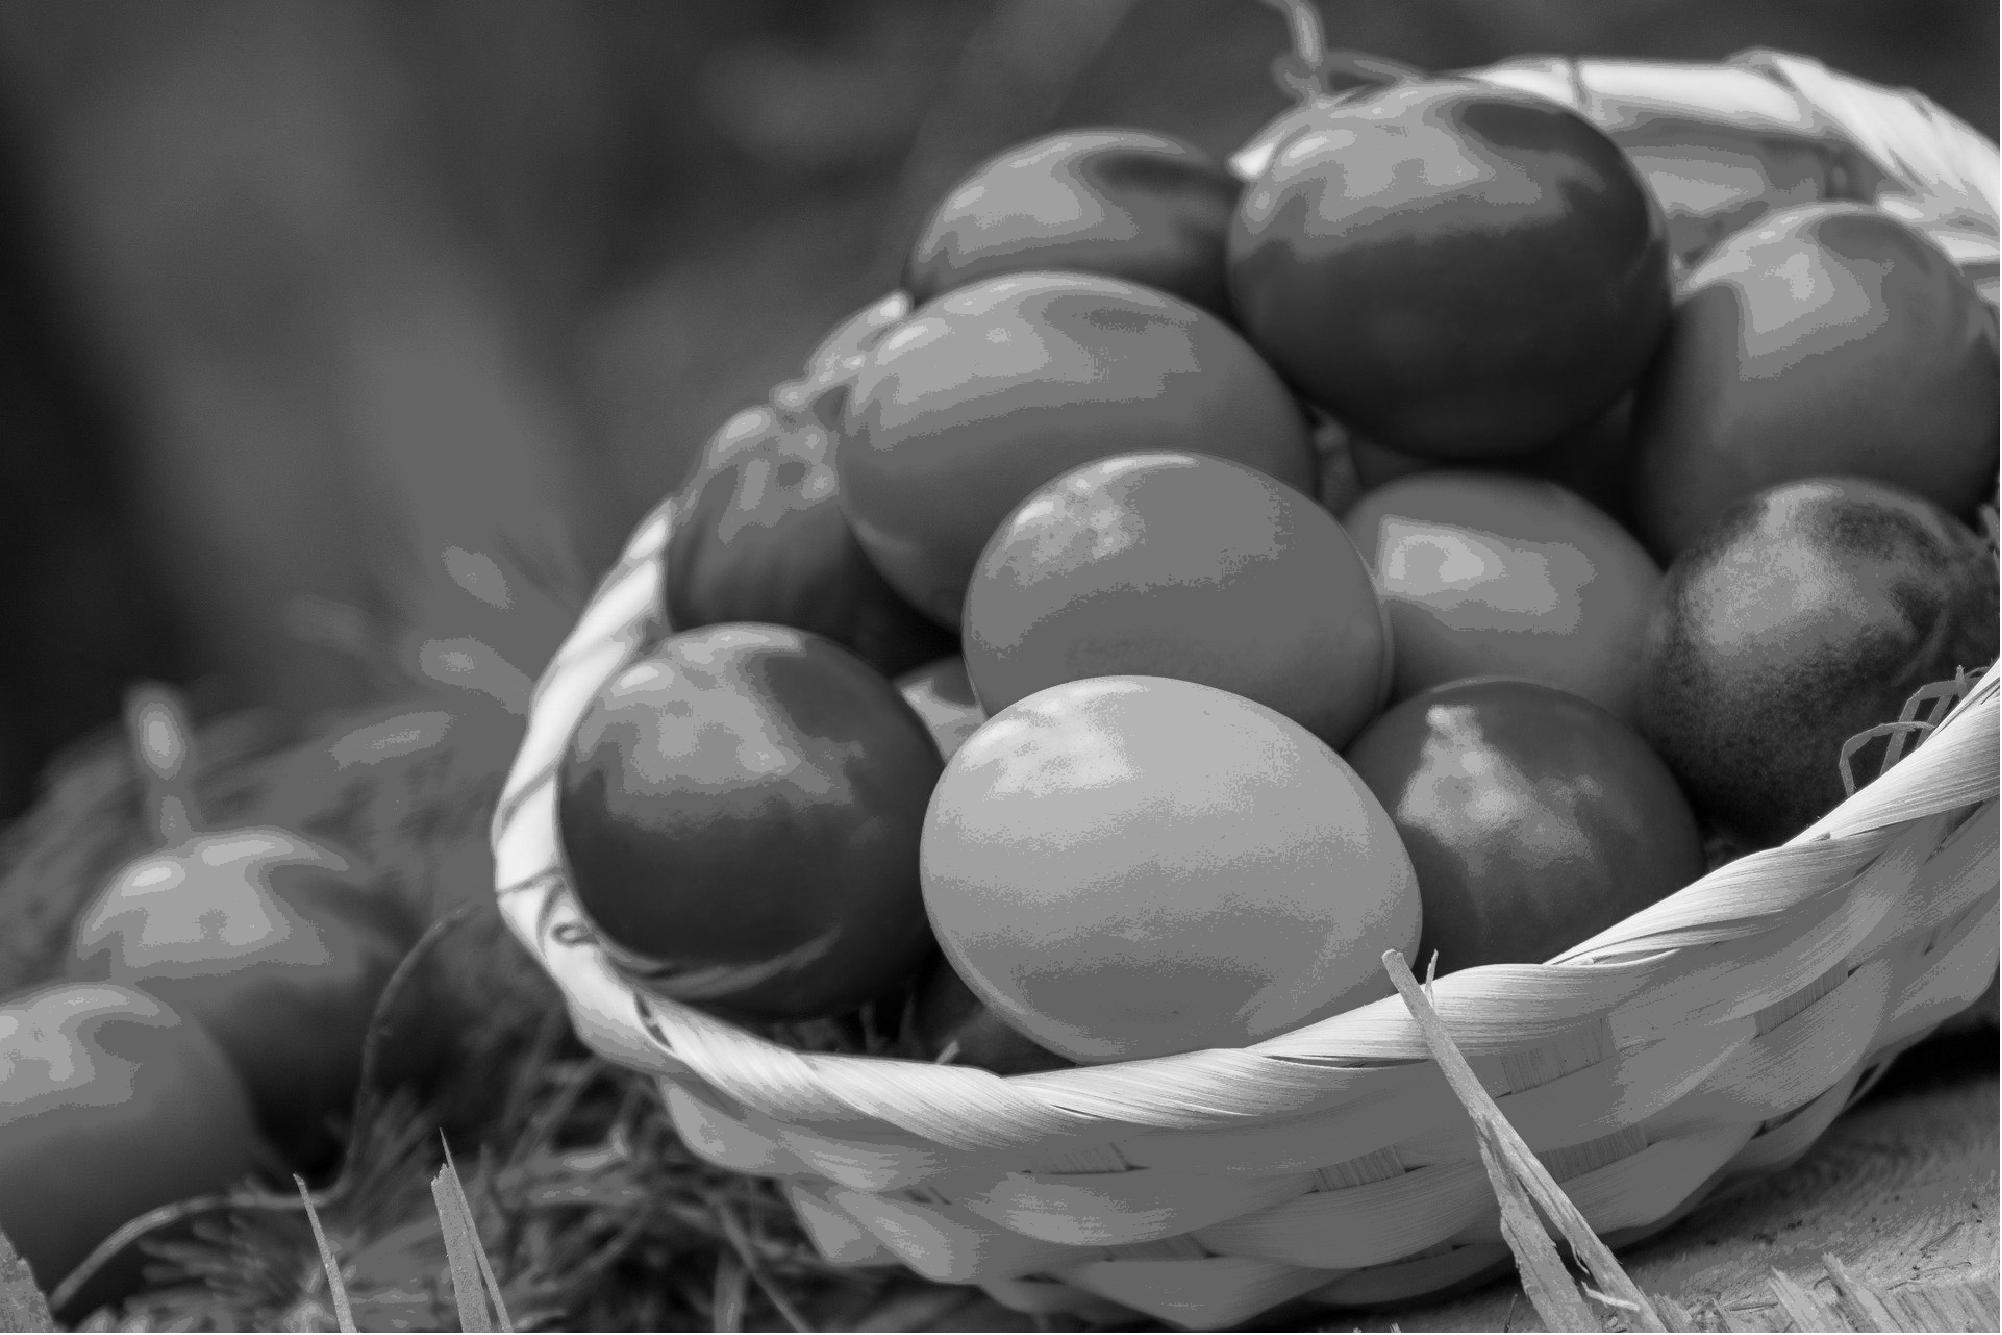
\includegraphics[width=1\linewidth]{kod matlab/myVectorFile13.pdf}
\caption{figure(13)}
    \label{fig:obr1}
\end{figure}

\begin{figure}[H]
    \centering
    \includegraphics[width=1\linewidth]{kod matlab/myVectorFile14.pdf}
\caption{figure(14)}
    \label{fig:obr1}
\end{figure}

\begin{figure}[H]
    \centering
    \includegraphics[width=1\linewidth]{kod matlab/myVectorFile15.pdf}
\caption{figure(15)}
    \label{fig:obr1}
\end{figure}

\begin{figure}[H]
    \centering
    \includegraphics[width=1\linewidth]{kod matlab/myVectorFile16.pdf}
\caption{figure(16)}
    \label{fig:obr1}
\end{figure}

\begin{figure}[H]
    \centering
    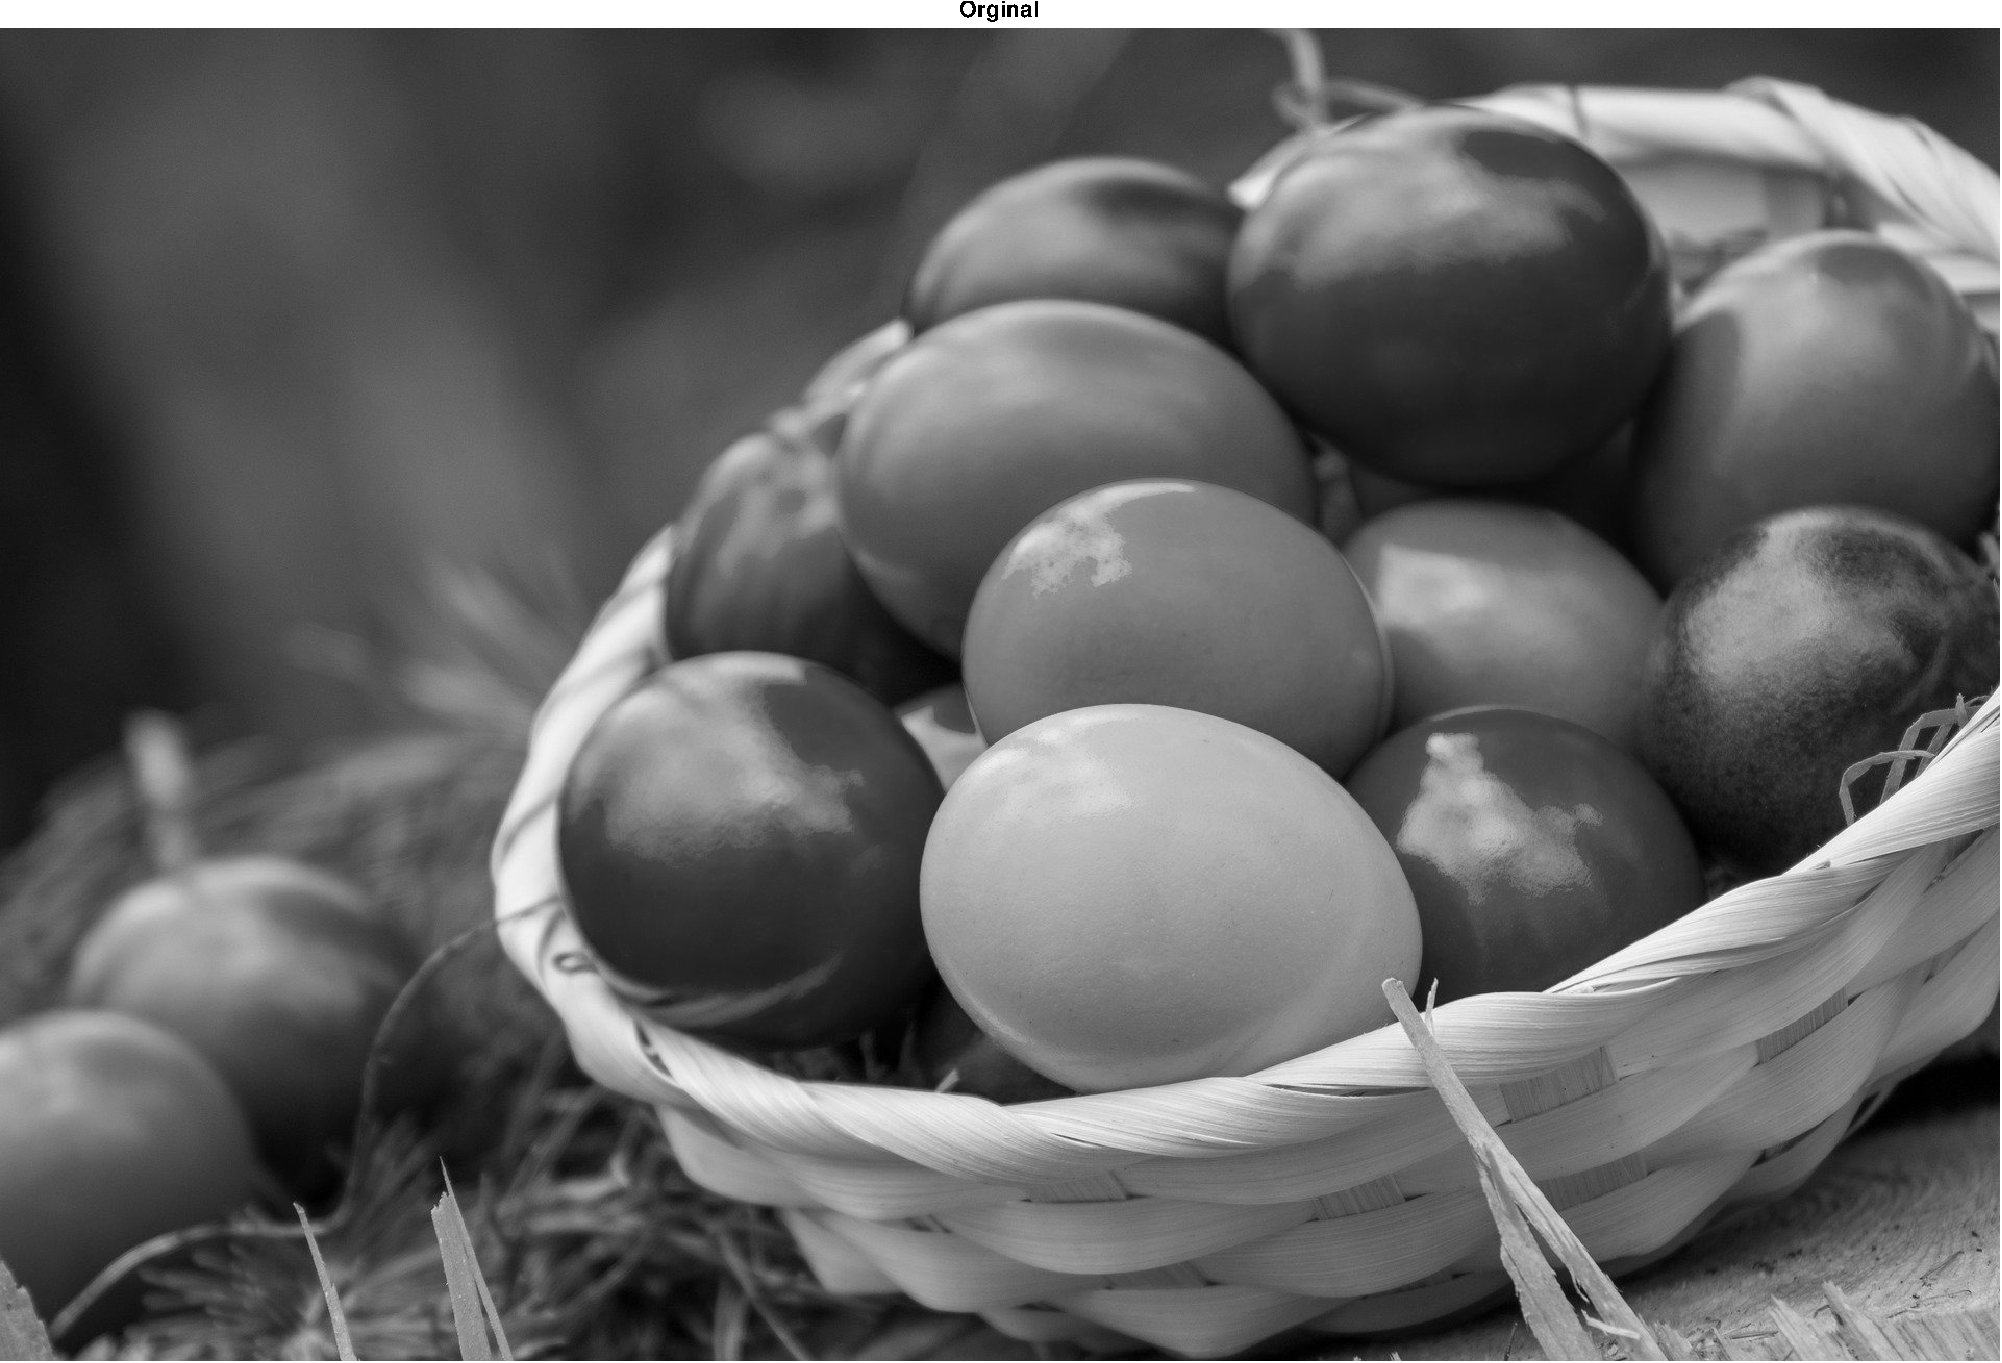
\includegraphics[width=1\linewidth]{kod matlab/myVectorFile17.pdf}
\caption{figure(17)}
    \label{fig:obr1}
\end{figure}

\begin{figure}[H]
    \centering
    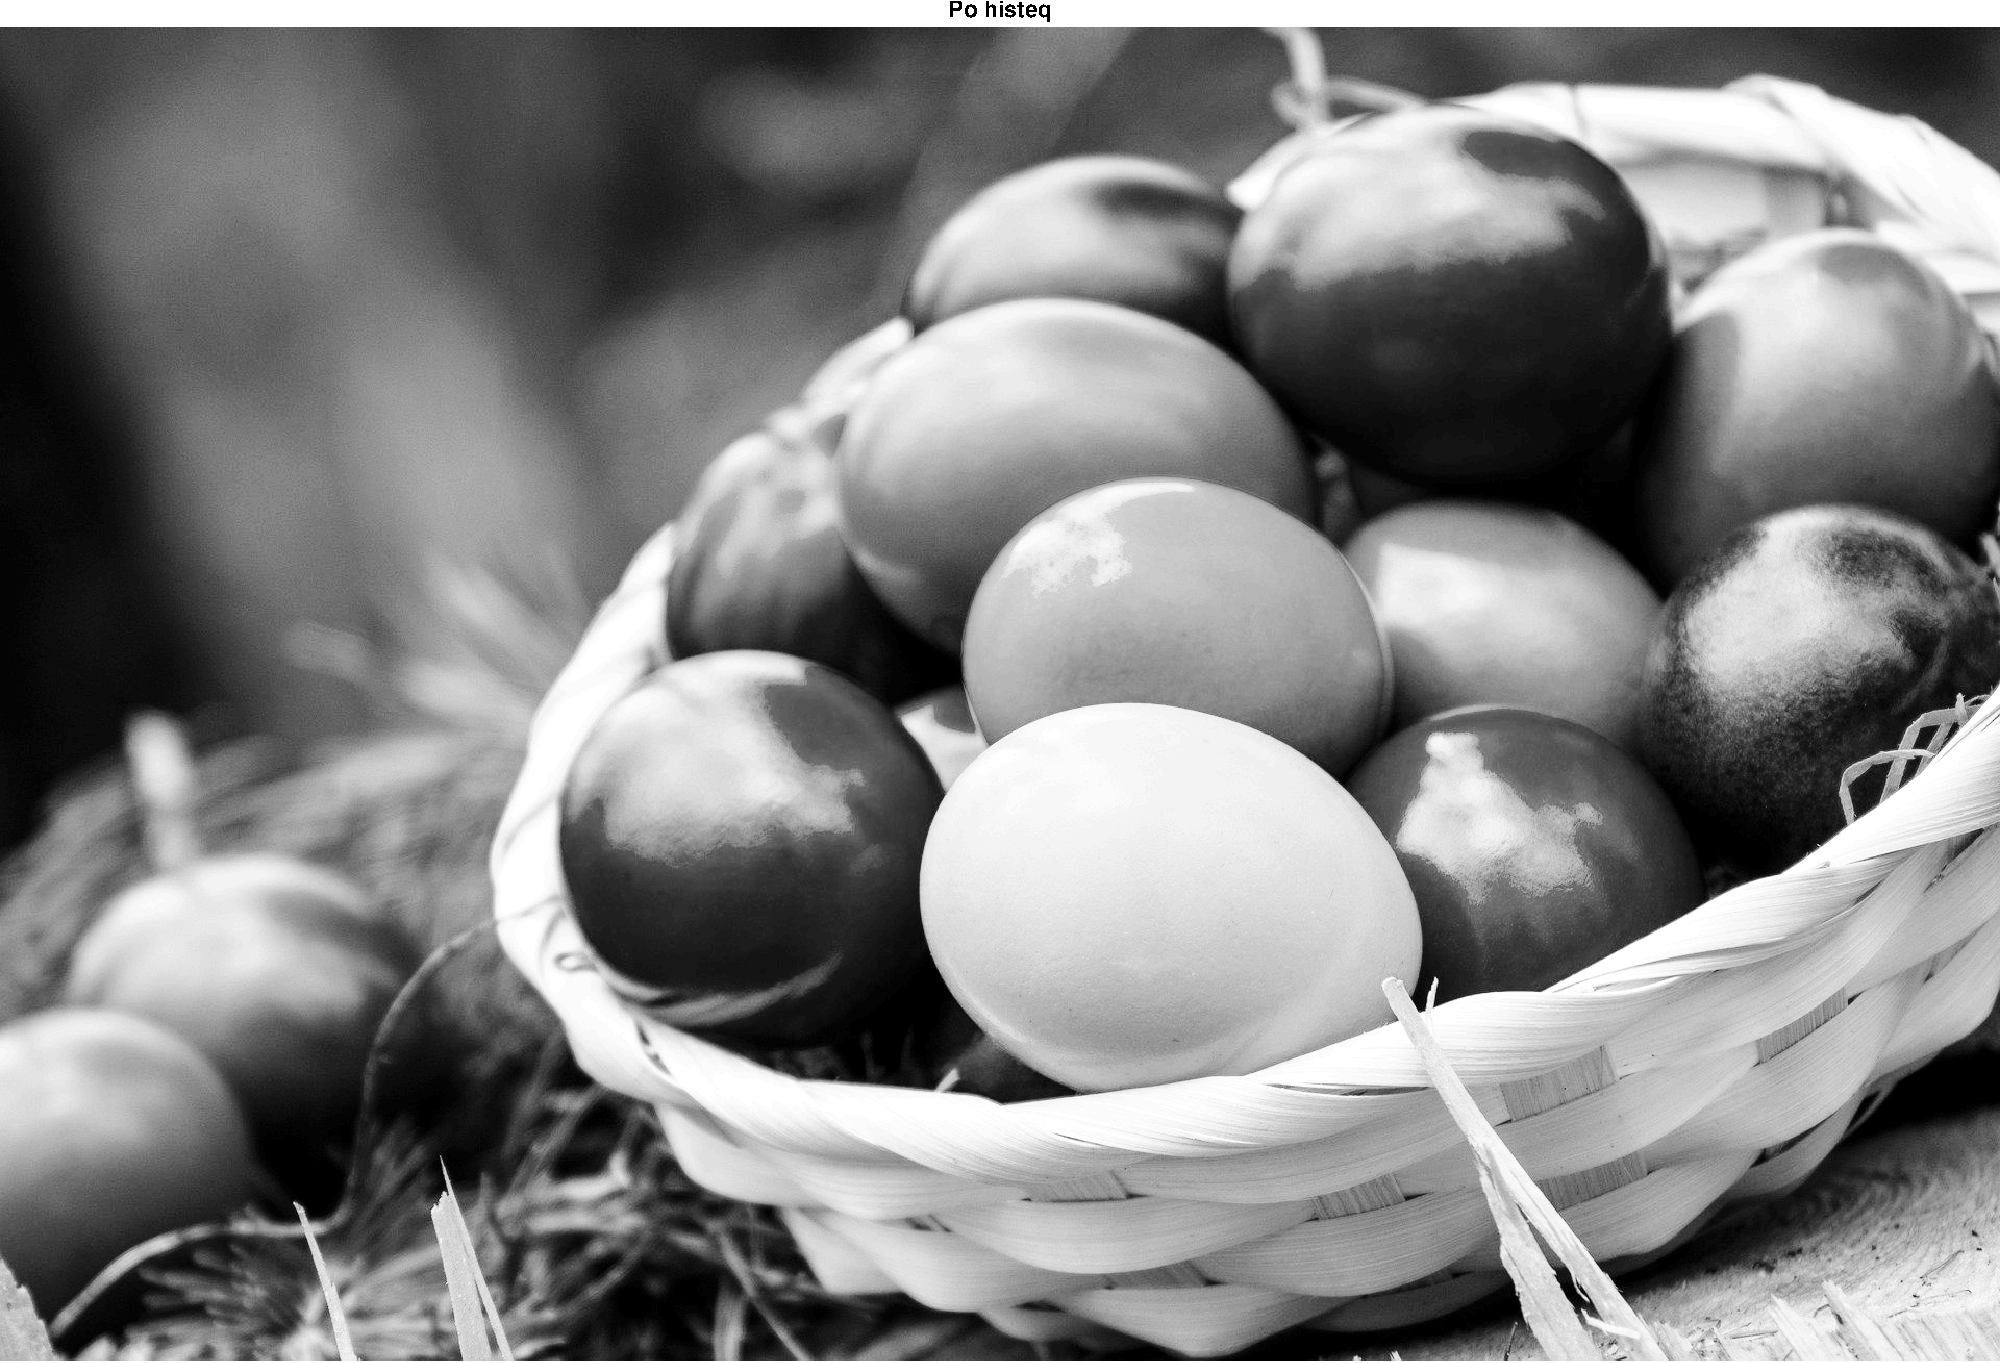
\includegraphics[width=1\linewidth]{kod matlab/myVectorFile18.pdf}
\caption{figure(18)}
    \label{fig:obr1}
\end{figure}

\begin{figure}[H]
    \centering
    \includegraphics[width=1\linewidth]{kod matlab/myVectorFile19.pdf}
\caption{figure(19)}
    \label{fig:obr1}
\end{figure}

\begin{figure}[H]
    \centering
    \includegraphics[width=1\linewidth]{kod matlab/myVectorFile20.pdf}
\caption{figure(20)}
    \label{fig:obr1}
\end{figure}

\begin{figure}[H]
    \centering
    \includegraphics[width=1\linewidth]{kod matlab/myVectorFile21.pdf}
\caption{figure(21)}
    \label{fig:obr1}
\end{figure}

\begin{figure}[H]
    \centering
    \includegraphics[width=1\linewidth]{kod matlab/myVectorFile22.pdf}
\caption{figure(22)}
    \label{fig:obr1}
\end{figure}

\begin{figure}[H]
    \centering
    \includegraphics[width=1\linewidth]{kod matlab/myVectorFile23.pdf}
\caption{figure(23)}
    \label{fig:obr1}
\end{figure}

\begin{figure}[H]
    \centering
    \includegraphics[width=1\linewidth]{kod matlab/myVectorFile24.pdf}
\caption{figure(24)}
    \label{fig:obr1}
\end{figure}

\begin{figure}[H]
    \centering
    \includegraphics[width=1\linewidth]{kod matlab/myVectorFile25.pdf}
\caption{figure(25)}
    \label{fig:obr1}
\end{figure}

\begin{figure}[H]
    \centering
    \includegraphics[width=1\linewidth]{kod matlab/myVectorFile26.pdf}
\caption{figure(26)}
    \label{fig:obr1}
\end{figure}

\begin{figure}[H]
    \centering
    \includegraphics[width=1\linewidth]{kod matlab/myVectorFile27.pdf}
\caption{figure(27)}
    \label{fig:obr1}
\end{figure}

\begin{figure}[H]
    \centering
    \includegraphics[width=1\linewidth]{kod matlab/myVectorFile28.pdf}
\caption{figure(28)}
    \label{fig:obr1}
\end{figure}

\begin{figure}[H]
    \centering
    \includegraphics[width=1\linewidth]{kod matlab/myVectorFile29.pdf}
\caption{figure(29)}
    \label{fig:obr1}
\end{figure}

\begin{figure}[H]
    \centering
    \includegraphics[width=1\linewidth]{kod matlab/myVectorFile30.pdf}
\caption{figure(30)}
    \label{fig:obr1}
\end{figure}

\begin{figure}[H]
    \centering
    \includegraphics[width=1\linewidth]{kod matlab/myVectorFile31.pdf}
\caption{figure(31)}
    \label{fig:obr1}
\end{figure}


\section{Wnioski}
Podsumowując, histogram jest ważnym narzędziem w przetwarzaniu obrazów, umożliwiającym między innymi wyznaczanie granicy binarnizacji. W tym kontekście, metoda Otsu jest wykorzystywana do znajdowania optymalnej granicy, a dołek na histogramie pomiędzy dwoma wzniesieniami ułatwia tę pracę. Zastosowano tutaj funkcje dostępne w środowisku Matlab: im2bw i imbinarize do binaryzacji obrazu oraz graythresh do wyznaczania granicy. Prowadzone przekształcenia obrazu, takie jak progowanie, mogą przynosić interesujące efekty wizualne i ograniczać ilość używanych odcieni, co jest dobrze widoczne na histogramach. Również wyrównanie histogramu może znacznie poprawić kontrast obrazu. Dyskutowano też operacje morfologiczne, takie jak erozja i dylatacja, które choć proste w swej naturze, potrafią wygenerować wyraźne efekty. Istotnym elementem jest tutaj dobór odpowiednich elementów strukturalnych, które różnią się w zależności od kierunku (np. poziome vs pionowe). Te operacje mogą służyć do usuwania szumów, bez usuwania cennych informacji z obrazu. Omówiono także operacje otwarcia i zamknięcia, które mogą być użyte do wypełniania nieciągłości figur. Proste operacje liniowe z wynikami erozji i dylatacji mogą w efekcie tworzyć kontury na obrazie. Istnieje możliwość manipulacji, by wygenerować kontury wewnętrzne (poprzez odjęcie erozji od oryginału) lub zewnętrzne (poprzez odjęcie dylatacji od oryginału).

\end{document}
